\documentclass[11pt,a4paper]{article}
\usepackage[T1]{fontenc}
\usepackage[utf8]{inputenc}
\usepackage{newtxtext,newtxmath}
\usepackage[scaled=0.94]{helvet}
\usepackage[margin=2.15cm,top=2.1cm,bottom=2.0cm]{geometry}
\usepackage{microtype,amsmath,mathtools,bm}
\usepackage{booktabs,tabularx,array,longtable,multicol}
\usepackage[dvipsnames]{xcolor}
\usepackage{tikz,pgfplots}
\pgfplotsset{compat=1.18}
\usetikzlibrary{arrows.meta,positioning,calc}
\usepackage[most]{tcolorbox}
\usepackage{enumitem,listings,fancyhdr,titlesec,needspace,tocloft}
\usepackage{hyperref}
\definecolor{navy}{HTML}{142C46}
\definecolor{teal}{HTML}{007F86}
\definecolor{pale}{HTML}{EEF6F6}
\definecolor{warm}{HTML}{FFF6E5}
\definecolor{graytext}{HTML}{52606D}
\hypersetup{colorlinks=true,linkcolor=navy,urlcolor=teal,citecolor=teal,pdftitle={Quantum Imaginary-Time Evolution: A Learning Guide},pdfauthor={OpenAI},pdfsubject={QITE, molecular ground states, numerical linear algebra and quantum Krylov benchmarks}}
\urlstyle{same}
\setlength{\parindent}{0pt}
\setlength{\parskip}{5pt}
\linespread{1.06}
\setlist[itemize]{leftmargin=1.5em,itemsep=2pt,topsep=3pt}
\setlist[enumerate]{leftmargin=1.7em,itemsep=3pt,topsep=3pt}
\setcounter{tocdepth}{1}
\setlength{\cftbeforesecskip}{4pt}
\renewcommand{\cftsecfont}{\small}
\renewcommand{\cftsecpagefont}{\small}
\setlength{\cftsecnumwidth}{1.8em}
\titleformat{\section}{\Large\sffamily\bfseries\color{navy}}{\thesection}{0.6em}{}
\titleformat{\subsection}{\large\sffamily\bfseries\color{teal}}{}{0em}{}
\titlespacing*{\section}{0pt}{0pt}{12pt}
\titlespacing*{\subsection}{0pt}{10pt}{4pt}
\pagestyle{fancy}
\fancyhf{}
\fancyhead[L]{\small\sffamily\color{graytext}QUANTUM IMAGINARY-TIME EVOLUTION}
\fancyhead[R]{\small\sffamily\color{graytext}Learning notes}
\fancyfoot[L]{\small\sffamily\color{graytext}Theory \; / \; worked examples \; / \; experiment design}
\fancyfoot[R]{\small\sffamily\thepage}
\renewcommand{\headrulewidth}{0.3pt}
\setlength{\headheight}{14pt}
\newcommand{\ket}[1]{\lvert #1\rangle}
\newcommand{\bra}[1]{\langle #1\rvert}
\newcommand{\braket}[2]{\langle #1\vert #2\rangle}
\newcommand{\ex}[1]{\langle #1\rangle}
\newcommand{\norm}[1]{\left\lVert #1\right\rVert}
\newcommand{\Var}{\operatorname{Var}}
\newcommand{\Rea}{\operatorname{Re}}
\newcommand{\Ima}{\operatorname{Im}}
\newcommand{\Tr}{\operatorname{Tr}}
\newcommand{\dd}{\mathrm{d}}
\newcommand{\dt}{\Delta\tau}
\newcommand{\Eh}{E_{\mathrm h}}
\newcommand{\lesson}[2]{\clearpage\section{#1}\label{#2}}
\newtcolorbox{idea}[1][Main idea]{enhanced,breakable,colback=pale,colframe=teal,boxrule=.5pt,arc=1.4mm,left=9pt,right=9pt,top=6pt,bottom=6pt,title={#1},fonttitle=\sffamily\bfseries,coltitle=white}
\newtcolorbox{caution}[1][Important distinction]{enhanced,breakable,colback=warm,colframe=Goldenrod,boxrule=.5pt,arc=1.4mm,left=9pt,right=9pt,top=6pt,bottom=6pt,title={#1},fonttitle=\sffamily\bfseries,coltitle=navy,colbacktitle=Goldenrod!25}
\newcommand{\checkpoint}[1]{\begin{idea}[Pause and check]#1\end{idea}}
\lstset{language=Python,basicstyle=\ttfamily\footnotesize,keywordstyle=\color{navy}\bfseries,commentstyle=\color{graytext},stringstyle=\color{teal},showstringspaces=false,breaklines=true,frame=single,rulecolor=\color{teal!35},backgroundcolor=\color{black!2},columns=fullflexible,keepspaces=true,aboveskip=6pt,belowskip=6pt}
\pgfplotsset{qiteplot/.style={width=.94\linewidth,height=5.7cm,grid=major,grid style={black!12},tick label style={font=\small},label style={font=\small},legend style={font=\small,draw=none,fill=white},every axis plot/.append style={thick},scaled ticks=false}}

\begin{document}
\begin{titlepage}
\color{navy}
{\sffamily\small\bfseries A SELF-STUDY GUIDE \hfill OCTOBER 2026\par}
\vspace{1.6cm}
{\sffamily\fontsize{35}{40}\selectfont\bfseries Quantum\\Imaginary-Time\\Evolution\par}
\vspace{.5cm}
{\sffamily\fontsize{24}{29}\selectfont\color{teal}QITE\par}
\vspace{.8cm}
{\Large From ground-state filtering to quantum circuits,\\measured linear systems, and molecular benchmarks.\par}
\vspace{.8cm}
\begin{tcolorbox}[colback=pale,colframe=teal,boxrule=0pt,arc=1mm,left=13pt,right=13pt,top=15pt,bottom=15pt]
\[
\frac{e^{-\tau H}\ket{\psi_0}}{\norm{e^{-\tau H}\ket{\psi_0}}}
\quad\longrightarrow\quad \ket{E_0}
\]
\centering\sffamily\large
The filter is simple. Implementing it efficiently is the challenge.
\end{tcolorbox}
\vspace{.9cm}
\begin{tabularx}{\linewidth}{@{}X X@{}}
\textbf{Learn the physics} & \textbf{Understand the computation}\\[4pt]
Normalization, spectral gaps, energy descent, and ground-state overlap. & State-dependent unitary updates, Pauli measurements, regularization, and circuit cost.\\[12pt]
\textbf{Work through examples} & \textbf{Design a fair comparison}\\[4pt]
One qubit, an entangling two-qubit model, and an explicit $H_2$ Hamiltonian. & QITE versus a specified quantum Krylov method under matched resource budgets.
\end{tabularx}
\vfill
{\sffamily\small\color{graytext}Includes original derivations, checked ideal simulations, exercises with solutions, and a runnable Python companion. Numerical demonstrations are not hardware results.}
\end{titlepage}

\section*{How to use these notes}
\addcontentsline{toc}{section}{How to use these notes}
These notes start from the material in your question, but make its approximations and assumptions explicit. The goal is understanding rather than formal theorem proving. You need basic matrix algebra, eigenvectors, and complex numbers. The necessary quantum notation is introduced as it appears.

\begin{idea}[The complete story in four sentences]
Imaginary-time evolution suppresses excited-state amplitudes relative to lower-energy amplitudes. Normalization turns this into a flow of physical quantum states. QITE approximates each small normalized step by a unitary chosen for the \emph{current} state. Measurements determine a linear system whose solution specifies that unitary.
\end{idea}

\subsection*{Three passes through the material}
\textbf{First pass: build intuition.} Read Sections~\ref{sec:toolkit}--\ref{sec:onequbit}, then the two-qubit example in Section~\ref{sec:domain}. Do not worry about implementing the entire algorithm yet. You should be able to explain why the ground state survives and why the unitary has to depend on the state.

\textbf{Second pass: implement and diagnose.} Read Sections~\ref{sec:trotter}--\ref{sec:code}. Reproduce the one-qubit sign check before running a molecular Hamiltonian. Then vary the step size and the operator pool separately.

\textbf{Third pass: connect to your project.} Read Sections~\ref{sec:varqite}--\ref{sec:robustness}. Treat the hardware benchmark as a proposed experimental protocol, not as a prediction that either algorithm will win.

\subsection*{What the companion files contain}
The PowerPoint is a teaching companion with speaker notes. The Python script uses only NumPy, SciPy, and Matplotlib; it evaluates tiny statevectors exactly so that each algorithmic ingredient can be checked. The archive includes its plots, raw CSV data, and numerical checks. The \LaTeX{} source is self-contained: its plots are embedded as equations or numerical coordinates, and its references do not require a separate bibliography file.

\begin{caution}[Scope]
Here \textbf{QITE} primarily means the state-dependent, local-unitary construction associated with Motta and collaborators~\cite{motta}. \textbf{Variational QITE} is a related, but different, ansatz-based method~\cite{mcardle,yuan}. A benchmark must state which one it uses. We do not assume your colleague's exact Krylov algorithm, molecule settings, or Quantinuum backend are already known.
\end{caution}

\clearpage
\tableofcontents

\lesson{The problem and the minimum quantum toolkit}{sec:toolkit}
\subsection*{The target}
A Hamiltonian $H$ is a Hermitian matrix describing the energy of a system. Its eigenpairs satisfy
\[
H\ket{E_n}=E_n\ket{E_n},\qquad E_0\le E_1\le\cdots.
\]
The molecular ground-state problem asks for the lowest energy in the \emph{chosen physical sector}, such as a fixed electron number and spin sector. A quantum algorithm may aim to prepare the ground state, estimate its energy, or both; these are not identical tasks.

\subsection*{States, basis vectors, and expectation values}
A normalized state is a complex column vector with $\braket{\psi}{\psi}=1$. For one qubit,
\[
\ket{0}=\begin{pmatrix}1\\0\end{pmatrix},\quad
\ket{1}=\begin{pmatrix}0\\1\end{pmatrix},\quad
\ket{\psi}=\alpha\ket{0}+\beta\ket{1},\quad
|\alpha|^2+|\beta|^2=1.
\]
The computational basis for two qubits is $\ket{00},\ket{01},\ket{10},\ket{11}$. It is a convenient storage and measurement basis, not generally the energy eigenbasis. With $N$ qubits, the statevector has $2^N$ entries.

For a normalized state, the energy and its variance are
\[
E=\bra{\psi}H\ket{\psi},\qquad
\Var_\psi(H)=\bra{\psi}H^2\ket{\psi}-E^2.
\]
A variance of zero says that the state lies in one energy eigenspace; it does \emph{not} say that this energy is the lowest.

\subsection*{The Pauli vocabulary}
\[
I=\begin{pmatrix}1&0\\0&1\end{pmatrix},\quad
X=\begin{pmatrix}0&1\\1&0\end{pmatrix},\quad
Y=\begin{pmatrix}0&-i\\i&0\end{pmatrix},\quad
Z=\begin{pmatrix}1&0\\0&-1\end{pmatrix}.
\]
A Pauli string is a tensor product, such as $X_0Z_1=X\otimes Z$. Any Hermitian qubit Hamiltonian has a real-coefficient expansion $H=\sum_{\alpha=1}^{L}h_\alpha P_\alpha$. Each Pauli string has measurement outcomes $+1$ and $-1$.

\begin{idea}[Notation used throughout]
$N$: system qubits; $L$: Hamiltonian terms; $D$: qubits in a QITE domain; $M$: generator-pool size; $\tau$: imaginary time; $\dt$: its step size; $K$: number of sweeps; $r$: Krylov subspace dimension. We use $\hbar=1$, so $\tau$ has units of inverse energy. $\Eh$ denotes one Hartree.
\end{idea}

\lesson{Why normalized imaginary time finds low energy}{sec:filter}
Write the normalized initial state in an orthonormal energy basis:
\[
\ket{\psi_0}=\sum_n c_n\ket{E_n},\qquad \sum_n|c_n|^2=1.
\]
Real-time evolution changes only phases: $c_n\mapsto c_ne^{-itE_n}$. It therefore leaves the probabilities $|c_n|^2$ unchanged. Imaginary-time evolution changes their relative magnitudes.

Define an unnormalized vector $\ket{\widetilde\psi(\tau)}=e^{-\tau H}\ket{\psi_0}$ and a normalized physical state
\begin{equation}
\boxed{\ket{\psi(\tau)}=
\frac{e^{-\tau H}\ket{\psi_0}}
{\sqrt{\bra{\psi_0}e^{-2\tau H}\ket{\psi_0}}}.}
\label{eq:normalized}
\end{equation}
Factoring out $e^{-\tau E_0}$ from both numerator and denominator gives
\[
\ket{\psi(\tau)}=
\frac{c_0\ket{E_0}+\sum_{n>0}c_ne^{-\tau(E_n-E_0)}\ket{E_n}}
{\sqrt{|c_0|^2+\sum_{n>0}|c_n|^2e^{-2\tau(E_n-E_0)}}}.
\]
For a nondegenerate ground state and $c_0\ne0$, this approaches $\ket{E_0}$ up to a physically irrelevant global phase. It is the \emph{normalized} state that converges; the raw vector can grow without bound or shrink toward zero.

The population of energy level $n$ is
\[
p_n(\tau)=\frac{|c_n|^2e^{-2\tau E_n}}{\sum_m |c_m|^2e^{-2\tau E_m}}.
\]
Thus the amplitude ratio decays with $e^{-\tau(E_n-E_0)}$, whereas the population ratio decays with $e^{-2\tau(E_n-E_0)}$. The factor of two matters.

\begin{caution}[Overlap and degeneracy]
If the initial state has no ground-state component, exact imaginary time cannot create one: it converges to the lowest-energy eigenspace already present in the initial state. If the ground energy is degenerate, the limit is the normalized projection of $\ket{\psi_0}$ into that ground space, not necessarily one particular eigenvector.
\end{caution}

\checkpoint{Why does real-time evolution alone not increase the ground-state population? Answer: it changes the phases of the coefficients, not their magnitudes.}

\lesson{Convergence speed, energy shifts, and assumptions}{sec:gap}
Assume a unique ground state and define the relevant gap $\Delta=E_1-E_0>0$ and initial ground population $p_0=|c_0|^2$. From the previous section,
\[
1-|\braket{E_0}{\psi(\tau)}|^2
\le \frac{1-p_0}{p_0}e^{-2\tau\Delta}.
\]
A sufficient time to make the infidelity at most $\varepsilon$ is therefore
\[
\tau\ge\frac{1}{2\Delta}
\log\!\left(\frac{1-p_0}{p_0\varepsilon}\right),
\]
with zero time sufficient when this bound is negative. This estimate is sufficient, not always tight. The relevant gap may be the gap within a symmetry sector rather than the gap of an unrestricted Hamiltonian.

\textbf{Interpretation.} A small gap slows filtering. A poor initial overlap also makes filtering harder. Moreover, a tiny overlap can make preparing or certifying a useful initial state difficult. None of this establishes that generic ground-state problems are efficiently solvable.

\subsection*{The zero of energy is arbitrary}
Let $H'=H-\lambda I$. Then
\[
e^{-\tau H'}=e^{\tau\lambda}e^{-\tau H},
\]
and the scalar factor cancels in Eq.~\eqref{eq:normalized}. Shifting energy changes neither the normalized trajectory nor energy gaps. It changes the reported energy by $-\lambda$.

\begin{caution}[A correction to a common explanation]
It is not generally true that $e^{-\tau E_n}<1$: negative energies give factors larger than one. The important fact is \emph{relative} suppression by $e^{-\tau(E_n-E_0)}$, independent of the energy origin. Non-unitarity means failure to preserve norms for arbitrary inputs, not necessarily norm decrease for every input.
\end{caution}

\subsection*{When energy error bounds state error}
For the same nondegenerate, gapped problem,
\[
E(\tau)-E_0\ge\Delta\bigl(1-|\braket{E_0}{\psi(\tau)}|^2\bigr).
\]
Hence small energy error certifies high ground-state fidelity only relative to a known positive gap. An energy tolerance alone does not specify a universal state-preparation accuracy.

\checkpoint{A constant term $h_I I$ in a molecular Hamiltonian affects the final energy. Does it affect the normalized QITE target direction? No: it cancels in $H-\ex{H}$.}

\lesson{Why a circuit cannot simply apply the filter}{sec:nonunitary}
A deterministic closed-system quantum circuit implements a unitary $U$, satisfying $U^\dagger U=I$. For Hermitian $H$,
\[
(e^{-\tau H})^\dagger e^{-\tau H}=e^{-2\tau H},
\]
which is not the identity for a generic nonzero Hamiltonian and $\tau>0$. The normalized map in Eq.~\eqref{eq:normalized} is also nonlinear as a function of the input vector because its normalization depends on that input.

\subsection*{A concrete obstruction}
Take $H=Z$. Normalized imaginary time leaves $\ket{0}$ unchanged, but transforms $\ket{+}=(\ket{0}+\ket{1})/\sqrt2$ into
\[
\frac{e^{-\tau}\ket{0}+e^{\tau}\ket{1}}
{\sqrt{e^{-2\tau}+e^{2\tau}}}.
\]
The magnitude of its overlap with $\ket{0}$ is no longer $1/\sqrt2$. A single unitary must preserve inner products between \emph{all} input states, so it cannot realize both transformations at once.

\begin{idea}[What QITE can ask for instead]
For one \emph{specified} normalized state and one normalized target, some unitary always connects them. QITE seeks a useful, approximately local, efficiently learnable version of that unitary. Its generator depends on the current state, the Hamiltonian term, and the allowed operator pool~\cite{motta}.
\end{idea}

\subsection*{Non-unitary operations are not forbidden in all quantum protocols}
An ancilla, a larger unitary circuit, and a measurement can produce a non-unitary transformation on a subsystem when conditioned on a measurement outcome. This introduces success probabilities and additional resources. Consequently, ``not an ordinary deterministic unitary on the system'' is more accurate than ``impossible on a quantum computer.''

The QITE construction developed here does not implement the exact filter by postselection at each step. It replaces a small \emph{normalized} state change by a state-dependent unitary learned from measurements. Other imaginary-time methods use different mechanisms and should not be treated as identical algorithms.

\checkpoint{Does $U\ket{\psi}\approx e^{-\dt H}\ket{\psi}/\norm{e^{-\dt H}\ket{\psi}}$ imply $U\approx e^{-\dt H}$ as operators? No. The approximation is about their action on one current state.}

\lesson{The normalized differential equation and energy descent}{sec:flow}
Let $\ket{\widetilde\psi}=e^{-\tau H}\ket{\psi_0}$ and $\mathcal N=\braket{\widetilde\psi}{\widetilde\psi}$. Direct differentiation gives
\[
\partial_\tau\ket{\widetilde\psi}=-H\ket{\widetilde\psi},\qquad
\partial_\tau\mathcal N=-2\mathcal N E.
\]
Differentiating $\ket{\psi}=\mathcal N^{-1/2}\ket{\widetilde\psi}$ yields
\begin{equation}
\boxed{\partial_\tau\ket{\psi}=-(H-E)\ket{\psi},\qquad E=\ex{H}.}
\label{eq:flow}
\end{equation}
The subtraction of $E$ removes the component that would only change the norm. In particular,
\[
\partial_\tau\braket{\psi}{\psi}=-2\ex{H-E}=0.
\]

For a time-independent Hamiltonian, differentiate $E=\bra{\psi}H\ket{\psi}$:
\begin{align*}
\frac{\dd E}{\dd\tau}
&=\bra{\partial_\tau\psi}H\ket{\psi}
 +\bra{\psi}H\ket{\partial_\tau\psi}\\
&=-\ex{(H-E)H}-\ex{H(H-E)}\\
&=-2(\ex{H^2}-E^2).
\end{align*}
\begin{equation}
\boxed{\frac{\dd E}{\dd\tau}=-2\Var_\psi(H)\le0.}
\label{eq:descent}
\end{equation}
The norm of the target tangent vector is also physically meaningful:
\[
\norm{(H-E)\ket{\psi}}^2=\Var_\psi(H).
\]
Large variance means a larger instantaneous imaginary-time change; zero variance means a stationary energy eigenstate.

\begin{caution}[Use the diagnostic correctly]
Exact continuous imaginary time is energy decreasing. Finite QITE steps, a restricted pool, Trotter splitting, inaccurate linear solves, and hardware or sampling errors need not give a perfectly monotone measured curve. Small upward fluctuations may be statistically harmless. Persistent increases merit investigation, not an automatic claim that the experiment is invalid.
\end{caution}

\lesson{QITE as a state-dependent tangent approximation}{sec:basic}
For a normalized current state, expand a small imaginary-time step:
\begin{align*}
\frac{e^{-\dt H}\ket{\psi}}{\norm{e^{-\dt H}\ket{\psi}}}
&=\bigl[I-\dt(H-E)\bigr]\ket{\psi}+O(\dt^2),\\
e^{-i\dt A}\ket{\psi}
&=\bigl[I-i\dt A\bigr]\ket{\psi}+O(\dt^2).
\end{align*}
Thus the first-order matching condition is
\begin{equation}
\boxed{iA\ket{\psi}\approx(H-E)\ket{\psi}.}
\label{eq:tangent}
\end{equation}
We choose a pool of Hermitian operators $\{\sigma_\mu\}_{\mu=1}^{M}$ and write
\[
A=\sum_{\mu=1}^{M}a_\mu\sigma_\mu,\qquad a_\mu\in\mathbb R.
\]
For ordinary Pauli-based QITE, the $\sigma_\mu$ are Pauli strings on a selected domain. Their real coefficients make $A$ Hermitian, so its exponential is unitary.

\begin{idea}[Do not equate the two operator lists]
The Hamiltonian strings $P_\alpha$ describe the energy. The generator strings $\sigma_\mu$ describe possible \emph{directions of state motion}. They need not be the same list. For $H=Z$ and $\ket{\psi}=\ket{+}$, the required generator is $Y$, not $Z$.
\end{idea}

\subsection*{Three levels to keep separate}
\textbf{Exact target:} the normalized filter in Eq.~\eqref{eq:normalized}.

\textbf{QITE approximation:} a fitted generator acting in an allowed operator span, derived by matching the first-order state change.

\textbf{Implemented circuit:} a synthesis of $e^{-i\dt A}$ into device gates. Gate synthesis can add another approximation even after $A$ has been determined.

After applying an update, the current state changes. The expectations and the fitted generator must generally be recomputed. In a term-by-term algorithm, replace $H$ in the local solve by the term being applied and use the state immediately before that term update.

\checkpoint{Why is a single generator, fitted only at $\tau=0$, generally insufficient? The correct tangent direction changes as the state changes.}

\lesson{Deriving the linear system without hiding the signs}{sec:linear}
Let $\ket{v}=(H-E)\ket{\psi}$. Minimize the squared tangent mismatch over \emph{real} coefficients:
\[
F(\bm a)=\norm{\ket{v}-i\sum_\mu a_\mu\sigma_\mu\ket{\psi}}^2.
\]
Expanding the square gives
\[
F(\bm a)=\Var_\psi(H)+\bm a^T S\bm a-2\bm a^T\bm b,
\]
where
\begin{align}
S_{\mu\nu}&=\Rea\bra{\psi}\sigma_\mu\sigma_\nu\ket{\psi}
=\tfrac12\ex{\{\sigma_\mu,\sigma_\nu\}},\label{eq:S}\\
b_\mu&=\Ima\bra{\psi}\sigma_\mu(H-E)\ket{\psi}
=\Ima\ex{\sigma_\mu H}.\label{eq:b}
\end{align}
The last equality follows because $E\ex{\sigma_\mu}$ is real. Differentiating with respect to each real coefficient yields
\begin{equation}
\boxed{S\bm a=\bm b.}
\label{eq:solve}
\end{equation}

\subsection*{Why $S$ is a Gram matrix}
For any real vector $\bm x$,
\[
\bm x^T S\bm x=\norm{\sum_\mu x_\mu\sigma_\mu\ket{\psi}}^2\ge0.
\]
Therefore $S$ is real symmetric and positive semidefinite in exact arithmetic. It can be singular because different operators may act identically on the current state. Nonunique coefficients need not imply a nonunique first-order state update.

\begin{caution}[Our convention is fixed]
These notes use $U=e^{-i\dt A}$, the residual $v-iA\psi$, and $b_\mu=\Ima\ex{\sigma_\mu H}$. Changing the sign in the unitary exponent changes the sign of the fitted generator. Some papers absorb factors of two, normalization constants, or a minus sign into their matrix definitions. Compare definitions before comparing printed equations~\cite{motta}.
\end{caution}

\subsection*{A useful residual}
After solving, report $r=\norm{(H-E)\psi-iA\psi}$. To first order, the local state error is $\dt\,r+O(\dt^2)$. Small time steps reduce discretization error, but they do not necessarily repair a pool that cannot represent the required tangent direction.

\lesson{What the linear algebra says about energy and locality}{sec:matrix}
\subsection*{Projected descent in the ideal continuous limit}
For the unitary tangent $\partial_\tau\ket{\psi}=-iA\ket{\psi}$,
\[
\frac{\dd E}{\dd\tau}=i\ex{[A,H]}=-2\bm a^T\bm b.
\]
With an exact solution of $S\bm a=\bm b$,
\[
\frac{\dd E}{\dd\tau}=-2\bm a^TS\bm a\le0.
\]
This is a property of the ideal projected \emph{continuous} flow for a solve using the full $H$. A finite circuit step need not inherit exact monotonicity. A local-term update descends that term in this sense, not necessarily the total Hamiltonian at every substep.

When $S$ is singular, a pseudoinverse gives the minimum-norm solution $\bm a=S^+\bm b$. In exact arithmetic, the least-squares minimum is
\[
F_{\min}=\Var_\psi(H)-\bm b^TS^+\bm b\ge0.
\]
A negative empirical estimate can indicate sampling or numerical inconsistency. Measuring this diagnostic can be expensive because it involves $H^2$.

\subsection*{An exact global generator exists, but is not an efficient recipe}
Define $\ket{v}=(H-E)\ket{\psi}$, so $\braket{\psi}{v}=0$, and set
\[
A_*=-i\bigl(\ket{v}\bra{\psi}-\ket{\psi}\bra{v}\bigr).
\]
Then $A_*$ is Hermitian and $iA_*\ket{\psi}=\ket{v}$. This elementary construction explains why the tangent can be represented with a sufficiently complete global pool.

\begin{idea}[Existence is not efficiency]
Writing $A_*$ explicitly requires information about the full state. Its Pauli expansion may be large and nonlocal. QITE becomes useful only when an adequately small domain or operator pool captures the required direction and can be measured and compiled at acceptable cost.
\end{idea}

\checkpoint{If $S$ is singular, should you add more shots until it becomes invertible? Not necessarily. Exact singularity often reflects redundant directions, not measurement error. Truncation or a pseudoinverse is the appropriate starting point.}

\lesson{A completely worked one-qubit example}{sec:onequbit}
Take $H=Z$ and $\ket{\psi_0}=\ket{+}$. The ground state is $\ket{1}$ with energy $-1$. Exact normalized evolution gives
\[
\ket{\psi(\tau)}=\frac{e^{-\tau}\ket{0}+e^{\tau}\ket{1}}
{\sqrt{e^{-2\tau}+e^{2\tau}}},\quad
E(\tau)=-\tanh(2\tau),\quad p_1(\tau)=\frac{1}{1+e^{-4\tau}}.
\]
At $\tau=0$, use the pool $(X,Y,Z)$. The Pauli anticommutation relations give $S=I_3$. Since $YZ=iX$ and $\ex{X}=1$,
\[
\bm b=(0,1,0)^T,\qquad\bm a=(0,1,0)^T,\qquad A=Y.
\]
For $\dt=0.1$, the QITE step is $e^{-i0.1Y}=R_y(0.2)$ and yields $E=-\sin(0.2)\approx-0.198669$. The exact one-step value is $-\tanh(0.2)\approx-0.197375$. They agree to the appropriate small-step order, but not exactly.

For a real state $\ket{\psi(\theta)}=\cos(\theta/2)\ket{0}+\sin(\theta/2)\ket{1}$, the fitted generator is $A=\sin\theta\,Y$. Thus a first-order update is $\theta\leftarrow\theta+2\dt\sin\theta$. The generator changes along the path.

\begin{center}
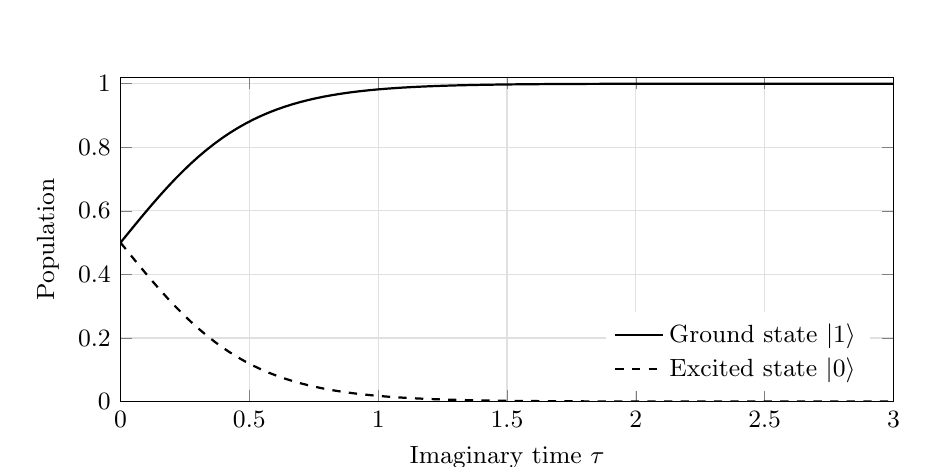
\begin{tikzpicture}
\begin{axis}[qiteplot,xmin=0,xmax=3,ymin=0,ymax=1.02,xlabel={Imaginary time $\tau$},ylabel={Population},legend pos=south east]
\addplot[domain=0:3,samples=100]{1/(1+exp(-4*x))};\addlegendentry{Ground state $\ket{1}$}
\addplot[dashed,domain=0:3,samples=100]{1/(1+exp(4*x))};\addlegendentry{Excited state $\ket{0}$}
\end{axis}
\end{tikzpicture}
\end{center}
\small\textit{Analytic curves derived above, not sampled hardware data.}\normalsize

\begin{idea}[Your first implementation test]
At $\ket{+}$ with $H=Z$, check that $a_Y=+1$ under our sign convention. A value of $-1$ drives the energy upward. A pool containing only $Z$ gives $b_Z=0$ and cannot follow the imaginary-time direction.
\end{idea}

\lesson{Domains, entanglement, and an instructive failure}{sec:domain}
A \emph{domain} is the set of qubits on which a local QITE update may act. A complete Pauli pool on $D$ qubits has at most $4^D$ strings including the identity. This exponential dependence is a central cost of the method~\cite{motta}.

Why might a local Hamiltonian term require a larger unitary domain? Non-unitary filtering can change correlations and Schmidt weights. A unitary acting only inside one small region cannot generally reproduce those changes. Enlarging the domain lets the update act on relevant correlations. Locality results rely on assumptions about correlations and accuracy; fixed small domains are not guaranteed for arbitrary molecular problems.

\subsection*{A two-qubit model where the issue is visible}
Consider the \emph{toy} Hamiltonian
\[
H=-Z_0-Z_1+0.6X_0X_1,\qquad \ket{\psi_0}=\ket{00}.
\]
Here $E(0)=-2$ and $(H-E)\ket{00}=0.6\ket{11}$. Single-qubit generators acting on $\ket{00}$ cannot produce the $\ket{11}$ direction. For the pool $\{X_0,Y_0,Z_0,X_1,Y_1,Z_1\}$, $\bm b=0$: QITE stalls at $-2$ even though the exact ground energy is $-\sqrt{4.36}\approx-2.0880613$.

A full two-qubit pool contains the missing direction. At the first step, one valid generator is $A=-0.3(X_0Y_1+Y_0X_1)$. It has $iA\ket{00}=0.6\ket{11}$.

\begin{center}
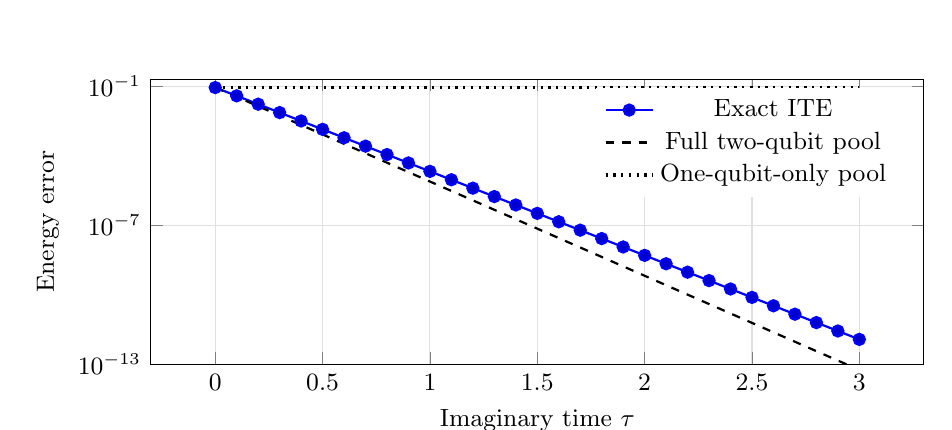
\begin{tikzpicture}
\begin{semilogyaxis}[qiteplot,height=5.2cm,xlabel={Imaginary time $\tau$},ylabel={Energy error},legend pos=north east,ymin=1e-13,ymax=.2]
\addplot coordinates {(0,0.08806130178) (0.1,0.03866057617) (0.2,0.01685844078) (0.3,0.007329558842) (0.4,0.003182557397) (0.5,0.001381116415) (0.6,0.0005992088513) (0.7,0.0002599441839) (0.8,0.0001127618029) (0.9,4.89142333e-05) (1,2.121801394e-05) (1.1,9.203914578e-06) (1.2,3.99245216e-06) (1.3,1.731835172e-06) (1.4,7.512305773e-07) (1.5,3.258666386e-07) (1.6,1.413534854e-07) (1.7,6.131590347e-08) (1.8,2.659743359e-08) (1.9,1.153735729e-08) (2,5.004640702e-09) (2.1,2.17089946e-09) (2.2,9.416858404e-10) (2.3,4.08482137e-10) (2.4,1.771898184e-10) (2.5,7.686118408e-11) (2.6,3.334088561e-11) (2.7,1.446176512e-11) (2.8,6.273648268e-12) (2.9,2.721378678e-12) (3,1.18038912e-12)};\addlegendentry{Exact ITE}
\addplot[dashed] coordinates {(0,0.08806130178) (0.1,0.03507826224) (0.2,0.01383567632) (0.3,0.005435601114) (0.4,0.002132147981) (0.5,0.0008358355266) (0.6,0.0003275818546) (0.7,0.0001283742413) (0.8,5.030601191e-05) (0.9,1.971313054e-05) (1,7.724828405e-06) (1.1,3.02706062e-06) (1.2,1.186186608e-06) (1.3,4.648199585e-07) (1.4,1.821446665e-07) (1.5,7.13753292e-08) (1.6,2.796918297e-08) (1.7,1.096002178e-08) (1.8,4.294801847e-09) (1.9,1.682963102e-09) (2,6.594866875e-10) (2.1,2.584270575e-10) (2.2,1.012674389e-10) (2.3,3.96833677e-11) (2.4,1.554978368e-11) (2.5,6.093792138e-12) (2.6,2.387423592e-12) (2.7,9.356959652e-13) (2.8,3.663735981e-13) (2.9,1.43884904e-13) (3,5.684341886e-14)};\addlegendentry{Full two-qubit pool}
\addplot[dotted,very thick,domain=0:3]{0.08806130178211};\addlegendentry{One-qubit-only pool}
\end{semilogyaxis}
\end{tikzpicture}
\end{center}
\small\textit{Ideal statevector calculations; full-pool QITE uses $\dt=0.05$. The restricted pool remains at its initial energy.}\normalsize

\checkpoint{Will a smaller step rescue the stalled one-qubit-only pool? No: it changes step length, not the span of accessible tangent directions.}

\lesson{Trotter splitting and accumulated circuit depth}{sec:trotter}
For $H=\sum_{\ell=1}^{L}h_\ell$, one common implementation uses a first-order product formula,
\[
e^{-\dt H}=e^{-\dt h_L}\cdots e^{-\dt h_2}e^{-\dt h_1}+O(\dt^2),
\]
where the rightmost factor acts first. Each normalized term update is approximated by its own fitted unitary. One pass through all $L$ terms is a \emph{sweep}, representing imaginary time $\dt$; after $K$ sweeps, $\tau=K\dt$, not $KL\dt$.

The order-$\dt^2$ one-sweep error depends on commutators and operator norms. Over fixed total time, a first-order formula generally accumulates order-$\dt$ error under suitable boundedness conditions. Term ordering and symmetric product formulas can change the discretization behavior.

\subsection*{Three separate approximations}
\begin{tabularx}{\linewidth}{@{}p{3.1cm}X@{}}
\toprule
Approximation & What is being replaced?\\\midrule
Hamiltonian splitting & $e^{-\dt\sum h_\ell}$ by a product of term filters.\\
QITE tangent fit & A normalized term filter by a state-dependent unitary from a chosen pool.\\
Unitary synthesis & $e^{-i\dt\sum a_\mu\sigma_\mu}$ by an implementable gate circuit.\\\bottomrule
\end{tabularx}

For example, a product of Pauli rotations,
\[
e^{-i\dt A}\approx\prod_\mu e^{-i\dt a_\mu\sigma_\mu},
\]
can add another product-formula error if the generator terms do not commute. The companion simulation instead exponentiates the small dense matrix $A$ exactly, so it does not model this error.

\begin{caution}[Local updates do not guarantee shallow prepared states]
After $s$ updates the state is $\ket{\psi_s}=U_s\cdots U_2U_1\ket{\psi_0}$. To measure it repeatedly, this \emph{whole preparation circuit} is generally rerun. Appending small local updates can therefore produce growing depth. Compression, gate cancellation, recompilation, or a fixed ansatz can help, but those are additional choices whose costs must be counted.
\end{caution}

Measuring a state normally consumes that preparation. QITE estimates many expectation values on repeated preparations; it does not preserve one measured copy and keep evolving it indefinitely.

\lesson{What must be measured, and what a shot buys}{sec:measurements}
For the Pauli expansion $H=\sum_\alpha h_\alpha P_\alpha$,
\[
E=\sum_\alpha h_\alpha\ex{P_\alpha},\quad
S_{\mu\nu}=\Rea\ex{\sigma_\mu\sigma_\nu},\quad
b_\mu=\sum_\alpha h_\alpha\Ima\ex{\sigma_\mu P_\alpha}.
\]
Products of Pauli strings reduce to a Pauli string times a phase in $\{1,-1,i,-i\}$. One does not need to measure a mysterious ``complex observable'': its real or imaginary part becomes a signed expectation of a Hermitian Pauli string.

For instance, $YZ=iX$ implies $\Ima\ex{YZ}=\ex{X}$. Anticommuting Hermitian Pauli strings have purely imaginary products, so they contribute zero to the real Gram matrix. Every Pauli-pool diagonal entry satisfies $S_{\mu\mu}=1$.

\subsection*{Basic measurement procedure}
Measure $Z$ directly. To measure $X$, apply a Hadamard before a computational-basis measurement. To measure $Y$, apply $S^\dagger$ and then a Hadamard, then measure. For a tensor-product string, combine the relevant single-qubit outcomes into their parity. Qubit-wise commuting strings can share a tensor-product measurement setting.

If a Pauli expectation $p$ is estimated from $n$ independent shots,
\[
\widehat p=\frac{n_+-n_-}{n},\qquad
\operatorname{SE}(\widehat p)=\sqrt{\frac{1-p^2}{n}}\le\frac{1}{\sqrt n}.
\]
For independently measured energy terms,
\[
\Var(\widehat E)=\sum_\alpha h_\alpha^2\frac{1-p_\alpha^2}{n_\alpha}.
\]
When terms share data, include their covariance rather than automatically using this independent-term formula.

\begin{idea}[Matrix entries are not the same as distinct measurements]
A naive calculation has $M^2$ Gram entries and $ML$ generator--Hamiltonian products. Many reduce to the same Pauli expectation, to zero, or to a known constant. Deduplicate before assigning shots. If all relevant operators live inside a $D$-qubit domain, there are at most $4^D$ distinct Pauli strings there; global-Hamiltonian products may require larger supports.
\end{idea}

A full Pauli pool has $M\sim4^D$. Dense storage of $S$ then scales like $M^2$, and a generic dense solve like $M^3$. These are implementation counts, not claims that every optimized QITE implementation must pay those costs.

\lesson{Solving a noisy Gram system and deciding when to stop}{sec:numerics}
The exact $S$ is positive semidefinite, but its estimate can be asymmetric or have small negative eigenvalues. A robust starting workflow is to symmetrize $\widehat S$, inspect its spectrum, and solve only within reliably resolved directions. Do not explicitly compute a matrix inverse.

\subsection*{Spectral cutoff}
Write $\widehat S=Q\operatorname{diag}(s_j)Q^T$. Keeping eigenvalues larger than a chosen threshold $\eta$ gives
\[
\bm a_\eta=\sum_{s_j>\eta}\frac{q_j^T\widehat{\bm b}}{s_j}q_j.
\]
The threshold should be reported and tested against the noise level. It trades information loss against noise amplification. Genuine large negative eigenvalues should trigger investigation rather than indiscriminate clipping.

\subsection*{Ridge penalty}
Adding $\lambda\norm{\bm a}^2$ to the tangent-fit objective produces
\[
(S+\lambda I)\bm a=\bm b,\qquad\lambda>0.
\]
This is a penalty on generator coefficients. It is \emph{not} the same objective as minimizing $\norm{S\bm a-\bm b}^2+\lambda\norm{\bm a}^2$, whose normal equations contain $S^TS$. Always specify which regularization is used.

\subsection*{A sensible stopping rule}
Use an energy-change threshold across several sweeps \emph{together with} uncertainty estimates and a resource ceiling. Where affordable, also inspect variance, tangent residual, retained rank, coefficient norm, and symmetry leakage. A flat curve can mean success, an inadequate pool, excessive regularization, an excited-state initial condition, or an unresolved signal.

\begin{caution}[Avoid selecting the best-looking noisy point]
The minimum among many noisy energy estimates is systematically optimistic. Choose the final state using a prespecified stopping rule, then evaluate it with independent measurements. Report uncertainty from repeated trajectories as well as the final energy measurement. A bootstrap of only the final measurement does not capture errors accumulated in earlier adaptive updates.
\end{caution}

A useful implementation check is to halve $\dt$ at fixed total $\tau$, then separately enlarge the pool. These test different approximations. Step size has units; $0.05\,\Eh^{-1}$ only makes sense together with the energy scale of the Hamiltonian.

\lesson{The complete hybrid loop}{sec:algorithm}
\begin{idea}[Inputs]
A Hamiltonian and its energy convention; an initial-state circuit; a decomposition into terms; a domain and operator pool per term; step size; maximum sweeps; a measurement plan; linear-solver thresholds; and stopping criteria.
\end{idea}

\begin{enumerate}
\item \textbf{Prepare and establish the reference.} Specify the physical symmetry sector and initial circuit. For small tests, calculate a classical reference energy from exactly the same Hamiltonian.
\item \textbf{At the start of a sweep,} the stored circuit prepares the current approximate state. For every Hamiltonian term $h_\ell$ in the chosen order, do the following.
\item \textbf{Measure the local system.} Generate and deduplicate the Pauli expectations needed for $S^{(\ell)}$ and $b^{(\ell)}$, evaluated on repeated preparations of the current state. Here $b_\mu^{(\ell)}=\Ima\ex{\sigma_\mu h_\ell}$.
\item \textbf{Solve classically.} Symmetrize the Gram matrix, apply the prespecified regularization, solve for $\bm a^{(\ell)}$, and log the retained rank, conditioning, and coefficient norm.
\item \textbf{Compile and append.} Form $A_\ell=\sum_\mu a_\mu^{(\ell)}\sigma_\mu$ and append an implementation of $e^{-i\dt A_\ell}$. Any later expectations in this sweep must use this updated state.
\item \textbf{After the sweep,} measure the full energy and other scheduled diagnostics; update $\tau\leftarrow\tau+\dt$. Check the stopping criterion and the cumulative resource budget.
\item \textbf{Validate the selected state.} Obtain an independent final energy estimate and report its uncertainty along with all training and evaluation costs.
\end{enumerate}

\subsection*{A simpler learning implementation}
For one to four qubits, first solve against the \emph{full} Hamiltonian with a global pool rather than splitting it into terms. This removes Trotter splitting as a source of confusion. It is the approach used in the companion demonstrations. It teaches the linear system correctly, but is not a scalable local-QITE hardware implementation.

\begin{caution}[What is classical and what is quantum?]
On hardware, the quantum device supplies expectation-value estimates and applies preparation circuits. A classical computer assembles the small fitted system, chooses coefficients, compiles circuits, and manages stopping. In the teaching script, both sides are replaced by exact dense linear algebra. No shot count or hardware runtime can be inferred from those statevector runs.
\end{caution}

\lesson{From a molecule to the qubit Hamiltonian}{sec:molecules}
For fixed nuclear geometry, a finite spin-orbital basis gives an electronic Hamiltonian of the form
\[
H_{\rm elec}=\sum_{pq}t_{pq}a_p^\dagger a_q
+\frac12\sum_{pqrs}v_{pqrs}a_p^\dagger a_q^\dagger a_s a_r,
\]
where $v_{pqrs}$ is defined consistently with the displayed prefactor and index order. Conventions vary, so use a chemistry package's definitions rather than mixing coefficients from different formulas. Nuclear repulsion is a scalar contribution:
\[
H_{\rm total}=H_{\rm elec}+E_{\rm nuc}I.
\]
Fermion-to-qubit transformations, such as Jordan--Wigner, convert this into Pauli strings. Occupation of spin orbitals becomes computational-basis information. The official OpenFermion tutorial provides a concrete electronic-structure workflow~\cite{openfermion}.

\subsection*{A reproducible preparation chain}
\begin{center}
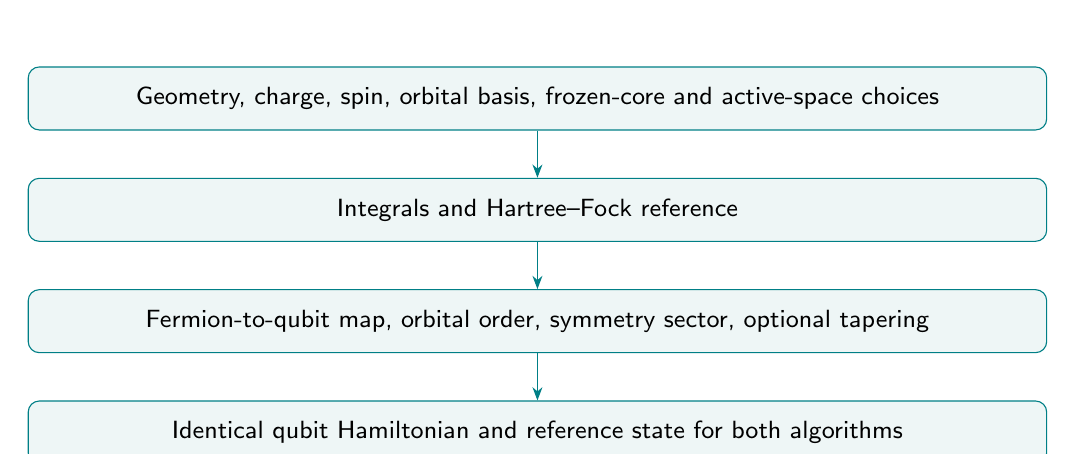
\begin{tikzpicture}[node distance=6mm,box/.style={draw=teal,fill=pale,rounded corners,text width=12.7cm,align=center,minimum height=8mm,font=\sffamily\small},arr/.style={-{Stealth},teal}]
\node[box](a){Geometry, charge, spin, orbital basis, frozen-core and active-space choices};
\node[box,below=of a](b){Integrals and Hartree--Fock reference};
\node[box,below=of b](c){Fermion-to-qubit map, orbital order, symmetry sector, optional tapering};
\node[box,below=of c](d){Identical qubit Hamiltonian and reference state for both algorithms};
\draw[arr](a)--(b);\draw[arr](b)--(c);\draw[arr](c)--(d);
\end{tikzpicture}
\end{center}

\textbf{Hartree--Fock (HF)} supplies a mean-field reference, commonly a computational-basis determinant after the occupation mapping. A larger correlation energy does not by itself determine the quality of HF's ground-state overlap.

\textbf{Full configuration interaction (FCI)} means exact diagonalization within the specified finite orbital space and physical sector. It is not the exact continuum molecular energy. An active-space FCI reference retains active-space and basis approximations.

\begin{caution}[Never compare different energy conventions]
Geometry, basis, active space, electron number, spin sector, mapping, orbital ordering, tapering values, frozen-core offsets, and nuclear repulsion must match. Do not add $E_{\rm nuc}$ twice when a supplied qubit Hamiltonian already includes it. The lowest eigenvalue across all occupation sectors need not be the desired molecular reference.
\end{caution}

\lesson{An explicit, reproducible hydrogen example}{sec:h2data}
The companion code uses the four-qubit Jordan--Wigner Hamiltonian from the official OpenFermion tutorial: neutral singlet $H_2$, inter-nuclear separation $0.8$~\AA, STO-3G basis, and four spin orbitals~\cite{openfermion}. The constant includes the nuclear contribution. The labels below are ordered $q_0q_1q_2q_3$, with $q_0$ the leftmost tensor factor.

\begin{center}
\small
\begin{tabular}{@{}lr@{\hspace{1.0cm}}lr@{}}
\toprule
Pauli string & Coefficient ($\Eh$) & Pauli string & Coefficient ($\Eh$)\\\midrule
IIII & $-0.1673339890569520$ & XXYY & $-0.0461566958890153$\\
XYYX & $+0.0461566958890153$ & YXXY & $+0.0461566958890153$\\
YYXX & $-0.0461566958890153$ & ZIII & $+0.1625164874887164$\\
ZZII & $+0.1658325372159041$ & ZIZI & $+0.1172036472019586$\\
ZIIZ & $+0.1633603430909739$ & IZII & $+0.1625164874887164$\\
IZZI & $+0.1633603430909739$ & IZIZ & $+0.1172036472019586$\\
IIZI & $-0.1974429369975584$ & IIZZ & $+0.1716978839228672$\\
IIIZ & $-0.1974429369975584$ & &\\\bottomrule
\end{tabular}
\end{center}
The code retains the source's precision. Preparing the HF state means $\ket{1100}$ in the stated convention, or entry 12 of a length-16 vector when basis indices follow ordinary binary order.

\subsection*{Check the reference before doing QITE}
Direct diagonalization and evaluation of the initial determinant give
\begin{align*}
E_{\rm HF}&=-1.110850397476595\,\Eh,\\
E_{\rm FCI}&=-1.134147666677096\,\Eh.
\end{align*}
These are \emph{computed} from the supplied coefficients. The ground state for this instance is in the desired two-electron sector. In general, explicitly enforce and check the sector rather than relying on that coincidence.

\subsection*{A real-state pool reduction}
This Hamiltonian and initial vector are real in the computational basis. Pauli strings with an odd number of $Y$ factors are purely imaginary Hermitian matrices; $-iA$ is then real and generates real-state motion. The example uses all such strings on four qubits, giving
\[
M=\frac{4^4-2^4}{2}=120.
\]
This is a complete pool for real antisymmetric generators, not a fixed small local pool. No claim of favorable scaling is implied. Its many redundant state-action directions are handled by a spectral pseudoinverse.

\lesson{What the hydrogen calculation actually demonstrates}{sec:h2results}
\begin{center}
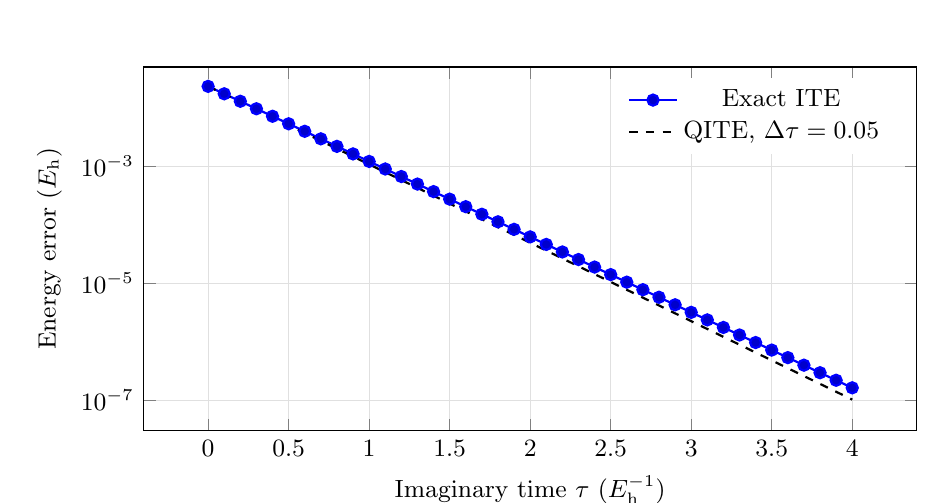
\begin{tikzpicture}
\begin{semilogyaxis}[qiteplot,height=6.2cm,xlabel={Imaginary time $\tau$ ($\Eh^{-1}$)},ylabel={Energy error ($\Eh$)},legend pos=north east,ymin=3e-8,ymax=.05]
\addplot coordinates {(0,0.0232972692) (0.1,0.01737597541) (0.2,0.01294633634) (0.3,0.009638531479) (0.4,0.007171761317) (0.5,0.005334026482) (0.6,0.003965941237) (0.7,0.002948047693) (0.8,0.002191019321) (0.9,0.001628174704) (1,0.001209799759) (1.1,0.000898865147) (1.2,0.0006678089289) (1.3,0.0004961266295) (1.4,0.0003685699758) (1.5,0.0002738027368) (1.6,0.0002033988507) (1.7,0.0001510963295) (1.8,0.0001122420019) (1.9,8.337848006e-05) (2,6.193702985e-05) (2.1,4.600925123e-05) (2.2,3.417737935e-05) (2.3,2.538817384e-05) (2.4,1.885921047e-05) (2.5,1.400925565e-05) (2.6,1.040653741e-05) (2.7,7.73031459e-06) (2.8,5.742326542e-06) (2.9,4.265583554e-06) (3,3.168610888e-06) (3.1,2.353744318e-06) (3.2,1.748435428e-06) (3.3,1.29879278e-06) (3.4,9.64784016e-07) (3.5,7.166717884e-07) (3.6,5.323662302e-07) (3.7,3.954582819e-07) (3.8,2.937587704e-07) (3.9,2.182131906e-07) (4,1.620955727e-07)};\addlegendentry{Exact ITE}
\addplot[dashed] coordinates {(0,0.0232972692) (0.1,0.01718318669) (0.2,0.0126586701) (0.3,0.009317342112) (0.4,0.006853543488) (0.5,0.005038848308) (0.6,0.003703351611) (0.7,0.002721112114) (0.8,0.001999012129) (0.9,0.001468330369) (1,0.001078419096) (1.1,0.0007919880277) (1.2,0.0005816016266) (1.3,0.0004270856142) (1.4,0.000313611009) (1.5,0.0002302810117) (1.6,0.0001690900143) (1.7,0.0001241574132) (1.8,9.116404303e-05) (1.9,6.693784541e-05) (2,4.914935772e-05) (2.1,3.608797149e-05) (2.2,2.649756697e-05) (2.3,1.945578331e-05) (2.4,1.428534889e-05) (2.5,1.048896288e-05) (2.6,7.701475298e-06) (2.7,5.654771635e-06) (2.8,4.151987555e-06) (2.9,3.048575038e-06) (3,2.23839972e-06) (3.1,1.64353262e-06) (3.2,1.206754602e-06) (3.3,8.860527181e-07) (3.4,6.505791403e-07) (3.5,4.776839906e-07) (3.6,3.507367099e-07) (3.7,2.575263964e-07) (3.8,1.890872605e-07) (3.9,1.388362207e-07) (4,1.019396862e-07)};\addlegendentry{QITE, $\Delta\tau=0.05$}
\end{semilogyaxis}
\end{tikzpicture}
\end{center}
\small\textit{Calculated for these notes with exact expectation values, a full four-qubit odd-$Y$ pool, and dense matrix exponentials. No hardware noise, finite shots, or gate-synthesis error.}\normalsize

\begin{tabularx}{\linewidth}{@{}X r@{}}
\toprule
Quantity & Value\\\midrule
Imaginary-time step & $0.05\,\Eh^{-1}$\\
Updates / total imaginary time & $80\;/\;4\,\Eh^{-1}$\\
Ideal QITE final energy & $-1.134147564737410\,\Eh$\\
Absolute energy error & $1.0194\times10^{-7}\,\Eh$\\
Reference ground energy & $-1.134147666677096\,\Eh$\\\bottomrule
\end{tabularx}

\subsection*{What you should conclude}
The implementation has the right sign and normalization, its chosen pool spans the required instantaneous directions for this example, and the energy approaches the reference in exact arithmetic. The QITE and exact-ITE curves need not coincide at finite step size; even an approximate trajectory can reach an accurate ground energy.

\subsection*{What you should not conclude}
This is not a Quantinuum result, a shot-cost prediction, an accuracy guarantee for larger molecules, or evidence of an advantage over Krylov. In fact, the HF trajectory for this tiny instance occupies only a two-dimensional invariant subspace. A noiseless two-vector real-time Krylov calculation already recovers its ground energy. That makes $H_2$ an excellent debugging problem, but a weak stand-alone scalability benchmark.

\begin{idea}[Provenance and reproducibility]
The archive contains \texttt{qite\_demo.py}, \texttt{results.json}, and CSV trajectories. The script checks the one-qubit generator sign, the toy-model stagnation, the $H_2$ reference energy, and the ideal $H_2$ energy bound. All plotted numerical curves come from those calculations.
\end{idea}

\lesson{Reading and running the reference implementation}{sec:code}
Run the companion script in an environment with NumPy, SciPy, and Matplotlib:
\begin{lstlisting}[language=bash]
python -m pip install -r requirements.txt
python qite_demo.py --output-dir results
\end{lstlisting}
The core of one step is shown below. The full script includes input validation, diagnostics, model definitions, and tests.
\begin{lstlisting}
# H: Hermitian Hamiltonian; psi: normalized state
# operators: array of Hermitian pool matrices, shape (M,d,d)
B = (operators @ psi).T  # column mu is sigma_mu |psi>
Hpsi = H @ psi
E = np.vdot(psi, Hpsi).real
S = (B.conj().T @ B).real
S = 0.5 * (S + S.T)
b = (B.conj().T @ Hpsi).imag

s, Q = np.linalg.eigh(S)
keep = s > max(1e-10 * s[-1], 1e-14)
a = Q[:, keep] @ ((Q[:, keep].T @ b) / s[keep])
A = np.einsum("m,mij->ij", a, operators)
residual = np.linalg.norm((Hpsi - E*psi) - 1j*(A @ psi))
psi_next = scipy.linalg.expm(-1j * dt * A) @ psi
psi_next /= np.linalg.norm(psi_next)
\end{lstlisting}

\textbf{Why form $B$?} It collects the vectors being compared in the least-squares fit. The matrix product $B^\dagger B$ generates all Gram entries without manually coding every Pauli product. This is a simulator convenience; hardware must estimate equivalent expectations.

\textbf{Why use an eigendecomposition?} $S$ is a symmetric Gram matrix. Small or zero eigenvalues identify redundant or unresolved directions. The code discards them rather than dividing by zero.

\textbf{Why renormalize after a unitary?} In exact arithmetic it is unnecessary. In a floating-point simulation it corrects tiny numerical drift. It does not model a physical postselection step.

\begin{caution}[The exponential wall remains in this teaching code]
The script stores $2^N$-component vectors and dense $2^N\times2^N$ operators. Its quantum expectations are computed classically. It is designed to make mistakes visible on small systems, not to deliver quantum speedup or a production hardware implementation. Tested here with NumPy 2.3.5 and Matplotlib 3.10.8; the script records versions in its result file.
\end{caution}

\lesson{Standard QITE, variational QITE, and VQE}{sec:varqite}
\textbf{State-dependent local-unitary QITE} fits an operator $A$ for each current state and appends its unitary update. The domain or pool is chosen explicitly. It replaces a nonlinear energy-minimization search with repeated linear tangent fits, but it can still suffer from large measurement requirements and poor local approximations~\cite{motta}.

\textbf{Variational imaginary-time evolution (VarQITE)} begins with a parameterized state $\ket{\psi(\bm\theta)}$. Instead of searching over local Pauli generators, it projects the target flow onto the ansatz tangent vectors $\ket{\partial_i\psi}$~\cite{mcardle,yuan}:
\[
\sum_j M_{ij}\dot\theta_j=C_i,
\]
\[
M_{ij}=\Rea\braket{\partial_i\psi}{\partial_j\psi},\qquad
C_i=-\Rea\bra{\partial_i\psi}(H-E)\ket{\psi}.
\]
These are the elementary McLachlan equations for a specified normalized state representation. Global-phase alignment or a projected, gauge-invariant tangent metric can modify the formulation; use one consistent convention. A simple numerical update is $\bm\theta\leftarrow\bm\theta+\dt\dot{\bm\theta}$.

\textbf{VQE} uses a parameterized circuit as well, but seeks low energy through an explicitly chosen classical optimization method. It does not have to reproduce an imaginary-time trajectory.

\begin{tabularx}{\linewidth}{@{}p{2.4cm}X X@{}}
\toprule
Method & Main object being chosen & Important limitation\\\midrule
Local QITE & Generator coefficients for appended updates & Domain size, repeated measurements, accumulated depth\\
VarQITE & Parameter velocity in an ansatz & Ansatz expressivity and tangent-metric conditioning\\
VQE & Circuit parameters minimizing energy & Optimization, sampling cost, and ansatz bias\\\bottomrule
\end{tabularx}

\begin{caution}[Software names matter]
A tutorial using a class named \texttt{VarQITE} implements a variational approach, not automatically the original local-unitary algorithm. The Qiskit Algorithms variational-time-evolution tutorial is useful for learning this separate formulation~\cite{qiskitvar}. Calling both methods simply ``QITE'' without reporting the formulation makes a benchmark ambiguous.
\end{caution}

Neither a solvable local linear system nor an ideal descent direction guarantees that the complete practical procedure will efficiently reach the global molecular ground state.

\lesson{Quantum Krylov: states first, a projected eigenproblem second}{sec:krylov}
A common real-time Krylov construction prepares
\[
\ket{\phi_j}=e^{-it_jH}\ket{\psi_0},\qquad j=0,\ldots,r-1.
\]
A trial state is a linear combination $\ket{\Phi}=\sum_j c_j\ket{\phi_j}$. Its Rayleigh quotient is
\[
\mathcal E(\bm c)=\frac{\bm c^\dagger\mathcal H\bm c}{\bm c^\dagger O\bm c},\quad
\mathcal H_{ij}=\bra{\phi_i}H\ket{\phi_j},\quad
O_{ij}=\braket{\phi_i}{\phi_j}.
\]
Stationarity gives the generalized eigenproblem
\begin{equation}
\boxed{\mathcal H\bm c=\varepsilon O\bm c.}
\label{eq:krylov}
\end{equation}
The quantum computer estimates the required overlaps and matrix elements; the small eigenproblem is solved classically. Real-time and other Krylov variants differ in basis construction and measurement protocols~\cite{cortes}.

\subsection*{Do not confuse the matrices}
The QITE Gram matrix $S$ describes \emph{operator-action tangent vectors at one state}. The Krylov overlap matrix $O$ describes \emph{different prepared basis states}. Both can be ill-conditioned, but their entries and their roles are different.

\subsection*{A stable projected solve}
First enforce Hermiticity. Diagonalize $O=W\operatorname{diag}(d_j)W^\dagger$, retain $d_j>\eta$, and define
\[
T=W_{\rm keep}\operatorname{diag}(d_j^{-1/2}),\qquad
H_{\rm white}=T^\dagger\mathcal H T.
\]
Now solve the ordinary Hermitian eigenproblem for $H_{\rm white}$. The overlap cutoff changes the effective subspace and must be reported. Noise sensitivity and thresholding are substantive parts of quantum subspace diagonalization~\cite{epperly}.

\begin{caution}[An energy estimate is not automatically a prepared state]
The eigenvector $\bm c$ specifies a linear combination of basis states. Obtaining $\varepsilon$ does not itself prepare that superposition on hardware. If your target is energy estimation, compare energy estimation costs; if it is state preparation, include the extra state-construction cost for methods that require it.
\end{caution}

\lesson{QITE and Krylov are distinct, but not unrelated}{sec:comparison}
\begin{tabularx}{\linewidth}{@{}p{3.0cm}X X@{}}
\toprule
Question & Local-unitary QITE & Real-time Krylov example\\\midrule
What is constructed? & A sequence of updated states & A set of basis states\\
Classical task & Repeated linear tangent fits & A projected eigenproblem\\
Key tuning choices & Time step, pool, domain, regularization & Times, subspace dimension, overlap cutoff\\
Typical sensitivity & Missing tangent directions; update noise & Near-dependent basis states; matrix noise\\
Physical final state? & Final preparation circuit is explicit & Ritz coefficients do not by themselves prepare a state\\\bottomrule
\end{tabularx}

\subsection*{The connection}
Classical power iteration applies a filter repeatedly. Classical Krylov methods use a span of repeated actions. Likewise, QITE states at selected imaginary times can supply a \emph{quantum Lanczos} subspace. The original QITE work also develops this connection~\cite{motta}. Therefore it is inaccurate to say that QITE and all forms of quantum Krylov are fundamentally unrelated.

For equally spaced exact real-time states,
\[
O_{ij}=\bra{\psi_0}e^{-i(t_j-t_i)H}\ket{\psi_0}.
\]
Such structure can reduce the number of distinct quantities in some implementations. Other protocols need different circuits. Do not assign a universal measurement count to ``Quantum Krylov'' without specifying the algorithm.

\subsection*{What an honest comparison avoids}
There is no general rule that QITE always has shallower complete circuits, that Krylov always takes fewer shots, or that either method is more robust on a particular processor. Those outcomes depend on the model, state, implementation, compiler, and resource definition.

\begin{idea}[A useful optional third arm]
After separately implementing QITE and your colleague's specified method, consider QITE-generated Lanczos as a hybrid comparison. It answers a different question: whether subspace extraction improves the value obtained from the imaginary-time states already generated. Count its extra matrix measurements rather than treating them as free.
\end{idea}

For the very small hydrogen example here, two noiseless real-time states span the populated invariant subspace. This explains its excellent ideal Krylov performance without predicting what will happen under finite sampling or on a larger molecule.

\lesson{A benchmark protocol that answers a real question}{sec:benchmark}
\begin{idea}[Primary research question]
For a fixed molecular Hamiltonian and a prespecified resource budget, how do a specified QITE implementation and a specified quantum Krylov implementation trade energy-estimation accuracy, circuit requirements, measurement cost, and robustness?
\end{idea}

\textbf{Freeze the common problem.} Use the same geometry, orbital basis, active space, energy offsets, electron and spin sectors, and starting-state policy. Record the exact Hamiltonian as machine-readable coefficients. Use the same backend target and compatible compilation/mitigation policies. Identical hyperparameters are not required; comparable and documented tuning effort is.

\textbf{Stage A: deterministic simulation.} Compare both methods to exact diagonalization of the selected sector. Separate statevector ITE, ideal QITE, and the actual Krylov algorithm. Vary QITE step size and pool; vary Krylov times, dimension, and overlap threshold. Record failures as well as successful settings.

\textbf{Stage B: finite sampling only.} Introduce shot noise with no device noise. This isolates the statistics of the QITE linear system and Krylov matrix reconstruction. Use independent repetitions of the \emph{whole} algorithm, not just repeated final measurements.

\textbf{Stage C: device-informed simulation.} Add the same justified, documented noise assumptions to both implementations. A noise model is only an approximation to hardware. Report where it does not include drift, correlations, or compilation-specific effects.

\textbf{Stage D: hardware.} Execute with an explicit device identifier, calibration window, compiler version, and native gate accounting. Interleave or randomize runs where practical to reduce confounding by drift. Separate raw estimates from mitigated estimates.

\textbf{Stage E: resource-normalized reporting.} Plot error and uncertainty against cumulative measured cost. Also report the probability of reaching a target tolerance within the budget, including failed trajectories and tuning/evaluation costs according to your declared accounting policy.

\begin{caution}[The colleague's configuration is still an input]
Before finalizing the comparison, obtain the exact Krylov basis, times, measurement circuit, regularization, molecule settings, and output target. A change from overlap-based Krylov to a sample-based variant, for example, changes what a fair measurement and resource comparison means.
\end{caution}

\lesson{Resource accounting: count executions, not just diagrams}{sec:resources}
For circuit setting $c$, let $n_c$ be its number of executions, $g_{2,c}$ its compiled two-qubit gate count, and $d_c$ its compiled depth. Useful total costs are
\[
N_{\rm shots}^{\rm total}=\sum_c n_c,\qquad
G_2^{\rm total}=\sum_c n_c g_{2,c},\qquad
D_{\max}=\max_c d_c.
\]
The sum runs over all settings, iterations, repetitions, calibration circuits, mitigation circuits, and independent final evaluations included by the benchmark's declared scope. Include postselection failures in attempted-shot cost.

\begin{tabularx}{\linewidth}{@{}p{3.5cm}X@{}}
\toprule
Metric & What to record\\\midrule
Energy accuracy & $|\widehat E-E_{\rm ref}|$, signed bias, confidence intervals, and repeated-run spread\\
Circuit requirements & Total/ancilla qubits, deepest circuit, native two-qubit gates per execution\\
Cumulative workload & Total shots, distinct settings, circuit executions, shot-weighted two-qubit gates\\
Time and platform cost & Device time where available; classical solve and compile time; billed or quoted platform cost\\
Robustness & Success probability, retained ranks, discarded modes, symmetry checks, and failed runs\\\bottomrule
\end{tabularx}

\subsection*{Why equal shots alone can be misleading}
One million executions of a five-gate circuit are not the same gate workload as one million executions of a five-hundred-gate circuit. Conversely, equal total two-qubit gates can hide different peak depths and sensitivity to state-preparation errors. Use more than one cost axis, or show an accuracy--cost frontier under explicit constraints.

\subsection*{Quantinuum-specific planning}
Use the selected backend's current native gates, compilation path, emulator options, and official cost estimator. Quantinuum's documentation provides system-specific job-submission and job-costing guidance~\cite{quantinuum,quantcost}. Do not substitute a universal shot-to-credit formula or assume that all Quantinuum systems share one workflow. Log the device, software versions, and estimator date.

\begin{caution}[Separate scientific time from waiting time]
Wall-clock time includes queueing, network latency, and scheduling. Report it separately from device execution time and classical computation. Adaptive QITE has sequential feedback costs that may matter even when each individual solve or circuit is small.
\end{caution}

\lesson{A practical robustness study and reporting checklist}{sec:robustness}
Start with a small pilot rather than an enormous parameter grid. The following values are illustrative \emph{starting choices}, not optimized or validated prescriptions.

\begin{tabularx}{\linewidth}{@{}p{3.1cm}X@{}}
\toprule
Factor & Pilot study\\\midrule
QITE time step & Try $0.02$, $0.05$, and $0.10\,\Eh^{-1}$ at a fixed total time; assess against the Hamiltonian scale.\\
QITE pool/domain & Compare at least one deliberately restricted pool with a larger validated pool.\\
Regularization & Test several cutoffs relative to estimated noise; record retained rank, not only the cutoff.\\
Krylov construction & Test increasing dimension and time ranges using the actual protocol's units and circuit synthesis.\\
Shot budgets & Use several cumulative budgets; give both algorithms a documented allocation and tuning policy.\\
Initial states & Start with HF, then test a prespecified alternative when the ground overlap or strong correlation is a concern.\\\bottomrule
\end{tabularx}

\subsection*{The central figure}
The main plot should have cumulative hardware cost on the horizontal axis and absolute energy error on the vertical axis, with uncertainty or repeated-run quantiles. State the reference Hamiltonian and physical sector in the caption. A second plot should show success probability at a chosen error tolerance versus budget. Do not connect an ideal-statevector error curve to a guessed hardware-cost axis.

\subsection*{Minimum run record}
Save the Hamiltonian hash, model metadata, initial-state circuit, random seeds, backend and compilation details, full hyperparameters, shot allocations, circuit-level native counts, intermediate energies, solver spectra/cutoffs, final independent evaluation, and the accounting of unsuccessful attempts. For QITE also save fitted generators; for Krylov save the measured projected matrices.

\begin{idea}[Choose a tolerance as a declared scientific target]
An illustrative threshold is $1.6\,\mathrm{m}\Eh$, where $1\,\mathrm{m}\Eh=10^{-3}\,\Eh$. The appropriate tolerance depends on the observable and scientific question. Being close to finite-basis FCI does not remove basis-set, active-space, or other chemistry-model errors.
\end{idea}

Scale beyond one easy $H_2$ instance by including multiple bond lengths and at least one larger active space that still admits a reliable classical reference. Avoid making a ``quantum advantage'' claim from toy systems or from ignoring the classical work used to select a good instance or pool.

\lesson{Common misconceptions and their repairs}{sec:faq}
\textbf{``The unnormalized state converges to $\ket{E_0}$.''} It need not converge as a vector. Normalize it, then take the limit; ground-space overlap and degeneracy still matter.

\textbf{``Imaginary time always shrinks every amplitude.''} Negative eigenvalues can produce growing amplitudes. Only ratios relative to lower energies determine the filter.

\textbf{``QITE discovers a unitary equal to $e^{-\dt H}$.''} It fits the action of a normalized step on one current state, not a universal operator identity.

\textbf{``Use exactly the Hamiltonian's Pauli strings for $A$.''} Those strings can miss the required direction. The one-qubit $H=Z$ example needs a $Y$ generator.

\textbf{``Small domains mean the final circuit stays shallow.''} The accumulated preparation circuit generally grows unless an explicit compression or ansatz restriction prevents it.

\textbf{``No nonlinear optimizer means no numerical difficulty.''} QITE can encounter singular Gram matrices, shot-amplified coefficients, domain bias, and costly repeated measurements.

\textbf{``A flat energy proves convergence to the ground state.''} An excited eigenstate is stationary. An inadequate pool can also stall away from any eigenstate, as the two-qubit example shows.

\textbf{``The exact energy-descent formula must hold pointwise in noisy data.''} It describes an ideal continuous flow. Finite steps and statistical uncertainty require a more careful diagnostic.

\textbf{``Krylov energies below FCI show a better answer.''} An exact physical state's energy is bounded below by the matching ground energy. Noisy projected matrices, mitigation estimators, or a mismatched reference can violate this variational picture without representing a lower physical ground state.

\textbf{``Matching total shots settles which algorithm is cheaper.''} Complete-circuit depth, native gates, ancillas, feedback, mitigation, and platform accounting can change the comparison.

\textbf{``The hydrogen demonstration proves the algorithm scales.''} It verifies a small implementation. The instance has a tiny populated invariant subspace and is not a meaningful stand-alone scalability claim.

\begin{idea}[Five questions that prevent most mistakes]
Which normalized state is the target? Which tangent directions are allowed? Which expectations were actually measured? Which circuit is rerun for every shot? Which full set of costs is being compared?
\end{idea}

\lesson{Exercises: explain, derive, and experiment}{sec:exercises}
\begin{enumerate}
\item \textbf{Relative filtering.} Let $H=\operatorname{diag}(-3,-1)$ and $\ket{\psi_0}=\ket{+}$. Find the normalized ground-state population after time $\tau$. Explain why both unnormalized amplitudes grow without preventing convergence.
\item \textbf{Energy shift.} Prove that $H\mapsto H+5I$ leaves the normalized trajectory and the vector $\bm b$ unchanged. What happens to the reported energy?
\item \textbf{One-qubit sign check.} For $H=Z$, $\ket{\psi}=\ket{+}$, and pool $(X,Y,Z)$, calculate $S$, $\bm b$, and the first generator. Show that the energy initially decreases.
\item \textbf{No initial overlap.} Use the same Hamiltonian but start in $\ket{0}$. Does exact imaginary time reach the ground state? What are the energy and its variance?
\item \textbf{A missing direction.} In the two-qubit toy example, compute $(H-E)\ket{00}$ and explain why one-qubit generators cannot reproduce it. Verify the proposed two-qubit generator.
\item \textbf{Gap and fidelity.} A normalized state's energy is $0.002\,\Eh$ above a nondegenerate ground energy. A rigorous lower bound on the gap is $0.2\,\Eh$. What lower bound follows for its ground-state population?
\item \textbf{Noise amplification.} Suppose $S=\operatorname{diag}(1,10^{-6})$ and $\bm b=(0.1,10^{-4})^T$. Calculate the unregularized coefficients and those obtained by discarding eigenvalues below $10^{-5}$. Explain the tradeoff.
\item \textbf{Gate workload.} Method A uses $2\times10^5$ shots with 40 two-qubit gates per shot. Method B uses $5\times10^4$ shots with 300 such gates per shot. Which uses fewer shots? Which uses fewer total two-qubit gate executions?
\item \textbf{Simulation investigation.} Run the toy model at several step sizes while holding total $\tau$ fixed. Compare with exact ITE at that \emph{same time}, not only with $E_0$. Then repeat with the restricted pool.
\item \textbf{Benchmark critique.} A report compares QITE on one geometry to Krylov on another, counts only final energy shots for QITE, and reports the lowest noisy energy from 100 attempts. Identify three problems and propose repairs.
\end{enumerate}

\begin{idea}[A self-study sequence]
First explain the one-qubit example without looking at the notes. Next implement the linear solve and pass its sign test. Then diagnose the toy-model failure. Finally reproduce the hydrogen reference and design the resource ledger before considering hardware execution.
\end{idea}

\lesson{Worked solutions and interpretation}{sec:solutions}
\textbf{1.} The unnormalized amplitudes are $e^{3\tau}/\sqrt2$ and $e^{\tau}/\sqrt2$. The lower-energy population is
\[
p_0(\tau)=\frac{e^{6\tau}}{e^{6\tau}+e^{2\tau}}=\frac{1}{1+e^{-4\tau}}.
\]
The ratio of excited to ground amplitude is $e^{-2\tau}$, so the growth of the overall norm is irrelevant after normalization.

\textbf{2.} $e^{-\tau(H+5I)}=e^{-5\tau}e^{-\tau H}$, and the scalar cancels. The extra term in $b_\mu$ is $5\Ima\ex{\sigma_\mu}=0$. All reported energies increase by $5$ in the chosen energy units.

\textbf{3.} $S=I_3$, $\bm b=(0,1,0)^T$, and $A=Y$. For a small step, $E'=-\sin(2\dt)$, so the initial derivative is $-2$, in agreement with $-2\Var_+(Z)=-2$.

\textbf{4.} The normalized state remains $\ket{0}$. Its energy is $+1$, its variance is zero, and its overlap with the ground state $\ket{1}$ is zero. A stationary state need not be the ground state.

\textbf{5.} $H\ket{00}=-2\ket{00}+0.6\ket{11}$, so the centered target is $0.6\ket{11}$. Single-qubit operators give only $\ket{00}$, $\ket{01}$, or $\ket{10}$ directions. Because $(X_0Y_1+Y_0X_1)\ket{00}=2i\ket{11}$, the generator $-0.3(X_0Y_1+Y_0X_1)$ has exactly the required $iA\ket{00}$.

\textbf{6.} $1-F_0\le(E-E_0)/\Delta\le0.002/0.2=0.01$. Thus $F_0\ge0.99$, under the stated gap and sector assumptions.

\textbf{7.} The unregularized result is $(0.1,100)^T$. The spectral cutoff gives $(0.1,0)^T$. Truncation prevents a tiny-eigenvalue direction from producing a huge coefficient, but deliberately abandons that direction's contribution.

\textbf{8.} B uses fewer shots. A uses $8\times10^6$ two-qubit gate executions, while B uses $1.5\times10^7$. Gate workload alone still does not specify peak depth, noise, or billed cost.

\textbf{9.} A complete-pool first-order QITE trajectory should approach exact ITE as $\dt$ is reduced sufficiently at fixed total time. Energy alone can hide trajectory differences. The restricted pool stays at $-2$ in this example regardless of step size because its fitted direction is zero.

\textbf{10.} Use the same Hamiltonian and geometry; count adaptive-learning measurements as well as final evaluation; and replace best-of-100 selection with a prespecified final-state rule and independent evaluation. Report all attempts and their variability, not only the best outcome.

\lesson{One-page formula sheet}{sec:cheatsheet}
\begin{idea}[Exact imaginary time]
\[
\ket{\psi(\tau)}=\frac{e^{-\tau H}\ket{\psi_0}}{\norm{e^{-\tau H}\ket{\psi_0}}},\quad
\partial_\tau\ket{\psi}=-(H-E)\ket{\psi},\quad
\frac{\dd E}{\dd\tau}=-2\Var(H).
\]
A ground-space component must be present initially. A shift by a scalar multiple of $I$ does not change the normalized path.
\end{idea}

\begin{idea}[QITE update: our sign convention]
\[
U=e^{-i\dt A},\qquad A=\sum_\mu a_\mu\sigma_\mu,\qquad
S\bm a=\bm b,
\]
\[
S_{\mu\nu}=\Rea\ex{\sigma_\mu\sigma_\nu},\qquad
b_\mu=\Ima\ex{\sigma_\mu H},\qquad
r=\norm{(H-E)\psi-iA\psi}.
\]
For term-by-term QITE, replace $H$ in the local solve by the current term and recompute using the current state. Do not reuse the Hamiltonian's string list blindly as the generator pool.
\end{idea}

\begin{idea}[Krylov energy extraction]
\[
\ket{\phi_j}=e^{-it_jH}\ket{\psi_0},\quad
O_{ij}=\braket{\phi_i}{\phi_j},\quad
\mathcal H_{ij}=\bra{\phi_i}H\ket{\phi_j},\quad
\mathcal H\bm c=\varepsilon O\bm c.
\]
Regularize unresolved overlap directions. State preparation from the Ritz coefficients can require additional work.
\end{idea}

\begin{idea}[The resource ledger]
\[
\epsilon_E=|\widehat E-E_{\rm ref}|,\qquad
N_{\rm shots}^{\rm total}=\sum_c n_c,\qquad
G_2^{\rm total}=\sum_c n_cg_{2,c},\qquad D_{\max}=\max_c d_c.
\]
Also record uncertainty, physical sector, qubits, native gate counts, distinct settings, tuning and mitigation overhead, feedback, and failures.
\end{idea}

\textbf{The mental model to keep:} the filter chooses a direction; a pool limits what can be represented; measurements estimate a Gram system; a classical solve selects a unitary update; the entire preparation circuit must be paid for again when the state is measured.

\clearpage
\section*{References and a guided reading order}
\addcontentsline{toc}{section}{References and a guided reading order}
Read the one-qubit example here first, then the main construction in [1]. Read [2] and [3] to understand why variational imaginary time is a distinct formulation. For your comparison, read [4] for real-time Krylov and [5] for conditioning. Use [6] to check chemistry conventions; [7]--[9] are implementation references, not evidence that one algorithm will outperform another.

All derivations and numerical illustrations in these notes are presented in a consistent notation; no figures from the papers are reproduced. Online documentation was checked on 8 October 2026. Hardware interfaces and costing policies can change.

\begin{thebibliography}{9}
\small
\bibitem{motta} M. Motta, C. Sun, A. T. K. Tan, M. J. O'Rourke, E. Ye, A. J. Minnich, F. G. S. L. Brand\~ao, and G. K.-L. Chan.
\emph{Determining eigenstates and thermal states on a quantum computer using quantum imaginary time evolution}. Nature Physics \textbf{16}, 205--210 (2020).
\url{https://arxiv.org/abs/1901.07653}.

\bibitem{mcardle} S. McArdle, T. Jones, S. Endo, Y. Li, S. C. Benjamin, and X. Yuan.
\emph{Variational ansatz-based quantum simulation of imaginary time evolution}. npj Quantum Information \textbf{5}, 75 (2019).
\url{https://arxiv.org/abs/1804.03023}.

\bibitem{yuan} X. Yuan, S. Endo, Q. Zhao, Y. Li, and S. C. Benjamin.
\emph{Theory of variational quantum simulation}. Quantum \textbf{3}, 191 (2019).
\url{https://quantum-journal.org/papers/q-2019-10-07-191/}.

\bibitem{cortes} C. L. Cortes and S. K. Gray.
\emph{Quantum Krylov subspace algorithms for ground and excited state energy estimation} (2021 preprint).
\url{https://arxiv.org/abs/2109.06868}.

\bibitem{epperly} E. N. Epperly, L. Lin, and Y. Nakatsukasa.
\emph{A theory of quantum subspace diagonalization}. SIAM Journal on Matrix Analysis and Applications \textbf{43}, 1263--1290 (2022).
\url{https://arxiv.org/abs/2110.07492}.

\bibitem{openfermion} Google Quantum AI, OpenFermion.
\emph{Quantum simulation of electronic structure}. Official tutorial; source of the $H_2$, $0.8$~\AA, STO-3G Hamiltonian used in the companion calculation.
\url{https://quantumai.google/openfermion/tutorials/intro_workshop_exercises}.

\bibitem{qiskitvar} Qiskit Algorithms contributors.
\emph{Variational Quantum Time Evolution}. Official community documentation; variational formulation, not automatically local-unitary QITE.
\url{https://qiskit-community.github.io/qiskit-algorithms/tutorials/11_VarQTE.html}.

\bibitem{quantinuum} Quantinuum.
\emph{Quantinuum Systems}. Official system and workflow documentation.
\url{https://docs.quantinuum.com/systems/}.

\bibitem{quantcost} Quantinuum.
\emph{Job Costing}. Official, system-specific costing guide. Verify applicability to the selected backend before budgeting a run.
\url{https://docs.quantinuum.com/systems/trainings/helios/getting_started/costing.html}.
\end{thebibliography}
\end{document}
